\documentclass[]{article}
\usepackage{lmodern}
\usepackage{amssymb,amsmath}
\usepackage{ifxetex,ifluatex}
\usepackage{fixltx2e} % provides \textsubscript
\ifnum 0\ifxetex 1\fi\ifluatex 1\fi=0 % if pdftex
  \usepackage[T1]{fontenc}
  \usepackage[utf8]{inputenc}
\else % if luatex or xelatex
  \ifxetex
    \usepackage{mathspec}
  \else
    \usepackage{fontspec}
  \fi
  \defaultfontfeatures{Ligatures=TeX,Scale=MatchLowercase}
\fi
% use upquote if available, for straight quotes in verbatim environments
\IfFileExists{upquote.sty}{\usepackage{upquote}}{}
% use microtype if available
\IfFileExists{microtype.sty}{%
\usepackage{microtype}
\UseMicrotypeSet[protrusion]{basicmath} % disable protrusion for tt fonts
}{}
\usepackage[margin=1in]{geometry}
\usepackage{hyperref}
\hypersetup{unicode=true,
            pdftitle={Reproducible Research Project 1},
            pdfauthor={Katie M Brown},
            pdfborder={0 0 0},
            breaklinks=true}
\urlstyle{same}  % don't use monospace font for urls
\usepackage{color}
\usepackage{fancyvrb}
\newcommand{\VerbBar}{|}
\newcommand{\VERB}{\Verb[commandchars=\\\{\}]}
\DefineVerbatimEnvironment{Highlighting}{Verbatim}{commandchars=\\\{\}}
% Add ',fontsize=\small' for more characters per line
\usepackage{framed}
\definecolor{shadecolor}{RGB}{248,248,248}
\newenvironment{Shaded}{\begin{snugshade}}{\end{snugshade}}
\newcommand{\KeywordTok}[1]{\textcolor[rgb]{0.13,0.29,0.53}{\textbf{#1}}}
\newcommand{\DataTypeTok}[1]{\textcolor[rgb]{0.13,0.29,0.53}{#1}}
\newcommand{\DecValTok}[1]{\textcolor[rgb]{0.00,0.00,0.81}{#1}}
\newcommand{\BaseNTok}[1]{\textcolor[rgb]{0.00,0.00,0.81}{#1}}
\newcommand{\FloatTok}[1]{\textcolor[rgb]{0.00,0.00,0.81}{#1}}
\newcommand{\ConstantTok}[1]{\textcolor[rgb]{0.00,0.00,0.00}{#1}}
\newcommand{\CharTok}[1]{\textcolor[rgb]{0.31,0.60,0.02}{#1}}
\newcommand{\SpecialCharTok}[1]{\textcolor[rgb]{0.00,0.00,0.00}{#1}}
\newcommand{\StringTok}[1]{\textcolor[rgb]{0.31,0.60,0.02}{#1}}
\newcommand{\VerbatimStringTok}[1]{\textcolor[rgb]{0.31,0.60,0.02}{#1}}
\newcommand{\SpecialStringTok}[1]{\textcolor[rgb]{0.31,0.60,0.02}{#1}}
\newcommand{\ImportTok}[1]{#1}
\newcommand{\CommentTok}[1]{\textcolor[rgb]{0.56,0.35,0.01}{\textit{#1}}}
\newcommand{\DocumentationTok}[1]{\textcolor[rgb]{0.56,0.35,0.01}{\textbf{\textit{#1}}}}
\newcommand{\AnnotationTok}[1]{\textcolor[rgb]{0.56,0.35,0.01}{\textbf{\textit{#1}}}}
\newcommand{\CommentVarTok}[1]{\textcolor[rgb]{0.56,0.35,0.01}{\textbf{\textit{#1}}}}
\newcommand{\OtherTok}[1]{\textcolor[rgb]{0.56,0.35,0.01}{#1}}
\newcommand{\FunctionTok}[1]{\textcolor[rgb]{0.00,0.00,0.00}{#1}}
\newcommand{\VariableTok}[1]{\textcolor[rgb]{0.00,0.00,0.00}{#1}}
\newcommand{\ControlFlowTok}[1]{\textcolor[rgb]{0.13,0.29,0.53}{\textbf{#1}}}
\newcommand{\OperatorTok}[1]{\textcolor[rgb]{0.81,0.36,0.00}{\textbf{#1}}}
\newcommand{\BuiltInTok}[1]{#1}
\newcommand{\ExtensionTok}[1]{#1}
\newcommand{\PreprocessorTok}[1]{\textcolor[rgb]{0.56,0.35,0.01}{\textit{#1}}}
\newcommand{\AttributeTok}[1]{\textcolor[rgb]{0.77,0.63,0.00}{#1}}
\newcommand{\RegionMarkerTok}[1]{#1}
\newcommand{\InformationTok}[1]{\textcolor[rgb]{0.56,0.35,0.01}{\textbf{\textit{#1}}}}
\newcommand{\WarningTok}[1]{\textcolor[rgb]{0.56,0.35,0.01}{\textbf{\textit{#1}}}}
\newcommand{\AlertTok}[1]{\textcolor[rgb]{0.94,0.16,0.16}{#1}}
\newcommand{\ErrorTok}[1]{\textcolor[rgb]{0.64,0.00,0.00}{\textbf{#1}}}
\newcommand{\NormalTok}[1]{#1}
\usepackage{longtable,booktabs}
\usepackage{graphicx,grffile}
\makeatletter
\def\maxwidth{\ifdim\Gin@nat@width>\linewidth\linewidth\else\Gin@nat@width\fi}
\def\maxheight{\ifdim\Gin@nat@height>\textheight\textheight\else\Gin@nat@height\fi}
\makeatother
% Scale images if necessary, so that they will not overflow the page
% margins by default, and it is still possible to overwrite the defaults
% using explicit options in \includegraphics[width, height, ...]{}
\setkeys{Gin}{width=\maxwidth,height=\maxheight,keepaspectratio}
\IfFileExists{parskip.sty}{%
\usepackage{parskip}
}{% else
\setlength{\parindent}{0pt}
\setlength{\parskip}{6pt plus 2pt minus 1pt}
}
\setlength{\emergencystretch}{3em}  % prevent overfull lines
\providecommand{\tightlist}{%
  \setlength{\itemsep}{0pt}\setlength{\parskip}{0pt}}
\setcounter{secnumdepth}{0}
% Redefines (sub)paragraphs to behave more like sections
\ifx\paragraph\undefined\else
\let\oldparagraph\paragraph
\renewcommand{\paragraph}[1]{\oldparagraph{#1}\mbox{}}
\fi
\ifx\subparagraph\undefined\else
\let\oldsubparagraph\subparagraph
\renewcommand{\subparagraph}[1]{\oldsubparagraph{#1}\mbox{}}
\fi

%%% Use protect on footnotes to avoid problems with footnotes in titles
\let\rmarkdownfootnote\footnote%
\def\footnote{\protect\rmarkdownfootnote}

%%% Change title format to be more compact
\usepackage{titling}

% Create subtitle command for use in maketitle
\newcommand{\subtitle}[1]{
  \posttitle{
    \begin{center}\large#1\end{center}
    }
}

\setlength{\droptitle}{-2em}

  \title{Reproducible Research Project 1}
    \pretitle{\vspace{\droptitle}\centering\huge}
  \posttitle{\par}
    \author{Katie M Brown}
    \preauthor{\centering\large\emph}
  \postauthor{\par}
      \predate{\centering\large\emph}
  \postdate{\par}
    \date{February 25, 2019}


\begin{document}
\maketitle

\subsubsection{Loading and Pre-processing
data}\label{loading-and-pre-processing-data}

In this section I will:

\begin{enumerate}
\def\labelenumi{\arabic{enumi}.}
\tightlist
\item
  Check for a directory and create on if it doesn't exist
\item
  Check for the zip file to be downloaded and create it if it doesn't
  exist
\item
  Check for to unzipped .csv file and unzip file if it doesn't exist
\item
  Read the data from .csv into a DF called activity
\item
  Look over the data and assess for transformations and other processing
\end{enumerate}

\begin{Shaded}
\begin{Highlighting}[]
\CommentTok{# Step 1:}
\ControlFlowTok{if}\NormalTok{(}\OperatorTok{!}\KeywordTok{file.exists}\NormalTok{(}\StringTok{"./data"}\NormalTok{)) \{}
      \KeywordTok{dir.create}\NormalTok{(}\StringTok{"./data"}\NormalTok{)}
\NormalTok{\}}

\CommentTok{# Step 2:}
\ControlFlowTok{if}\NormalTok{(}\OperatorTok{!}\KeywordTok{file.exists}\NormalTok{(}\StringTok{"./data/activity.zip"}\NormalTok{)) \{}
\NormalTok{      url <-}\StringTok{ 'https://d396qusza40orc.cloudfront.net/repdata%2Fdata%2Factivity.zip'}
      \KeywordTok{download.file}\NormalTok{(url, }\DataTypeTok{destfile =} \StringTok{'./data/activity.zip'}\NormalTok{,}\DataTypeTok{method=}\StringTok{'curl'}\NormalTok{ )}
\NormalTok{\}}

\CommentTok{# Step 3: }
\ControlFlowTok{if}\NormalTok{(}\OperatorTok{!}\KeywordTok{file.exists}\NormalTok{(}\StringTok{"./data/activity.csv"}\NormalTok{)) \{}
      \KeywordTok{unzip}\NormalTok{(}\StringTok{'./data/activity.zip'}\NormalTok{,}\DataTypeTok{exdir =} \StringTok{'./data'}\NormalTok{)}
\NormalTok{\}}

\CommentTok{# Step 4:}
\NormalTok{activity <-}\StringTok{ }\KeywordTok{read.csv}\NormalTok{(}\StringTok{'data/activity.csv'}\NormalTok{)}

\CommentTok{# Step 5:}
\KeywordTok{str}\NormalTok{(activity)}
\end{Highlighting}
\end{Shaded}

\begin{verbatim}
## 'data.frame':    17568 obs. of  3 variables:
##  $ steps   : int  NA NA NA NA NA NA NA NA NA NA ...
##  $ date    : Factor w/ 61 levels "2012-10-01","2012-10-02",..: 1 1 1 1 1 1 1 1 1 1 ...
##  $ interval: int  0 5 10 15 20 25 30 35 40 45 ...
\end{verbatim}

\begin{Shaded}
\begin{Highlighting}[]
\KeywordTok{names}\NormalTok{(activity)}
\end{Highlighting}
\end{Shaded}

\begin{verbatim}
## [1] "steps"    "date"     "interval"
\end{verbatim}

\begin{Shaded}
\begin{Highlighting}[]
\KeywordTok{head}\NormalTok{(activity)}
\end{Highlighting}
\end{Shaded}

\begin{verbatim}
##   steps       date interval
## 1    NA 2012-10-01        0
## 2    NA 2012-10-01        5
## 3    NA 2012-10-01       10
## 4    NA 2012-10-01       15
## 5    NA 2012-10-01       20
## 6    NA 2012-10-01       25
\end{verbatim}

\begin{Shaded}
\begin{Highlighting}[]
\KeywordTok{tail}\NormalTok{(activity)}
\end{Highlighting}
\end{Shaded}

\begin{verbatim}
##       steps       date interval
## 17563    NA 2012-11-30     2330
## 17564    NA 2012-11-30     2335
## 17565    NA 2012-11-30     2340
## 17566    NA 2012-11-30     2345
## 17567    NA 2012-11-30     2350
## 17568    NA 2012-11-30     2355
\end{verbatim}

\begin{Shaded}
\begin{Highlighting}[]
\CommentTok{# After seeing NAs in both head and tail, I decide to sum the non-NAs to verify}
\CommentTok{# I have data in the steps column}
\KeywordTok{sum}\NormalTok{(}\OperatorTok{!}\KeywordTok{is.na}\NormalTok{(activity}\OperatorTok{$}\NormalTok{steps))}
\end{Highlighting}
\end{Shaded}

\begin{verbatim}
## [1] 15264
\end{verbatim}

\begin{Shaded}
\begin{Highlighting}[]
\CommentTok{# Data looks good except for the "date" column. Changed to a date object here:}
\NormalTok{activity}\OperatorTok{$}\NormalTok{date <-}\StringTok{ }\KeywordTok{as.Date}\NormalTok{(activity}\OperatorTok{$}\NormalTok{date)}
\end{Highlighting}
\end{Shaded}

\subsubsection{What is mean total number of steps taken per
day?}\label{what-is-mean-total-number-of-steps-taken-per-day}

In this section I will:

\begin{enumerate}
\def\labelenumi{\arabic{enumi}.}
\tightlist
\item
  Calculate the total number of steps taken per day while ignoring NAs
\item
  Make a histogram of the total number of steps taken each day

  \begin{itemize}
  \tightlist
  \item
    First I will import appropriate libraries and color palette
  \item
    Then I will change options to allow for appropriate decimal output
  \item
    Finally, I will create the histogram using ggplot2
  \end{itemize}
\item
  Calculate and report the mean and median of the total number of steps
  taken per day
\end{enumerate}

\begin{Shaded}
\begin{Highlighting}[]
\CommentTok{# Step 1:}
\NormalTok{per_day <-}\StringTok{ }\KeywordTok{aggregate}\NormalTok{(activity[}\StringTok{"steps"}\NormalTok{], }\DataTypeTok{by=}\NormalTok{activity[}\StringTok{"date"}\NormalTok{], sum)}

\CommentTok{# Step 2:}
\KeywordTok{library}\NormalTok{(dplyr)}
\KeywordTok{library}\NormalTok{(RColorBrewer)}
\KeywordTok{library}\NormalTok{(ggplot2)}
\NormalTok{shades <-}\StringTok{ }\KeywordTok{brewer.pal}\NormalTok{(}\DecValTok{9}\NormalTok{, }\StringTok{"Purples"}\NormalTok{)[}\KeywordTok{c}\NormalTok{(}\DecValTok{5}\OperatorTok{:}\DecValTok{8}\NormalTok{)]}

\KeywordTok{options}\NormalTok{(}\DataTypeTok{digits =} \DecValTok{9}\NormalTok{)}

\KeywordTok{ggplot}\NormalTok{() }\OperatorTok{+}\StringTok{ }\KeywordTok{aes}\NormalTok{(per_day}\OperatorTok{$}\NormalTok{steps) }\OperatorTok{+}\StringTok{ }\KeywordTok{geom_histogram}\NormalTok{(}\DataTypeTok{binwidth=}\DecValTok{1000}\NormalTok{, }\DataTypeTok{colour=}\NormalTok{shades[}\DecValTok{2}\NormalTok{], }\DataTypeTok{fill=}\NormalTok{shades[}\DecValTok{1}\NormalTok{]) }\OperatorTok{+}
\StringTok{      }\KeywordTok{geom_vline}\NormalTok{(}\DataTypeTok{xintercept=}\KeywordTok{mean}\NormalTok{(per_day}\OperatorTok{$}\NormalTok{steps,}\DataTypeTok{na.rm =} \OtherTok{TRUE}\NormalTok{), }\DataTypeTok{lwd=}\DecValTok{1}\NormalTok{, }\DataTypeTok{linetype=}\DecValTok{2}\NormalTok{, }\DataTypeTok{color=}\NormalTok{shades[}\DecValTok{4}\NormalTok{]) }\OperatorTok{+}
\StringTok{      }\KeywordTok{geom_label}\NormalTok{(}\DataTypeTok{x=}\DecValTok{13200}\NormalTok{, }\DataTypeTok{y=}\DecValTok{8}\NormalTok{, }\KeywordTok{aes}\NormalTok{(}\DataTypeTok{fontface=}\DecValTok{2}\NormalTok{),}\DataTypeTok{color=}\NormalTok{shades[}\DecValTok{3}\NormalTok{], }
                \DataTypeTok{label =} \KeywordTok{paste}\NormalTok{(}\StringTok{'Mean:'}\NormalTok{,}\KeywordTok{format}\NormalTok{(}\KeywordTok{round}\NormalTok{(}\KeywordTok{mean}\NormalTok{(per_day}\OperatorTok{$}\NormalTok{steps, }\DataTypeTok{na.rm=}\OtherTok{TRUE}\NormalTok{), }\DecValTok{2}\NormalTok{), }\DataTypeTok{nsmall =} \DecValTok{2}\NormalTok{))) }\OperatorTok{+}
\StringTok{      }\KeywordTok{geom_label}\NormalTok{(}\DataTypeTok{x=}\DecValTok{13450}\NormalTok{, }\DataTypeTok{y=}\FloatTok{7.45}\NormalTok{, }\KeywordTok{aes}\NormalTok{(}\DataTypeTok{fontface=}\DecValTok{2}\NormalTok{),}\DataTypeTok{color=}\NormalTok{shades[}\DecValTok{3}\NormalTok{], }
                 \DataTypeTok{label =} \KeywordTok{paste}\NormalTok{(}\StringTok{'Median:'}\NormalTok{,}\KeywordTok{format}\NormalTok{(}\KeywordTok{round}\NormalTok{(}\KeywordTok{median}\NormalTok{(per_day}\OperatorTok{$}\NormalTok{steps, }\DataTypeTok{na.rm=}\OtherTok{TRUE}\NormalTok{), }\DecValTok{2}\NormalTok{), }\DataTypeTok{nsmall =} \DecValTok{2}\NormalTok{))) }\OperatorTok{+}
\StringTok{      }\KeywordTok{xlab}\NormalTok{(}\StringTok{"Steps per Day"}\NormalTok{) }\OperatorTok{+}
\StringTok{      }\KeywordTok{ylab}\NormalTok{(}\StringTok{""}\NormalTok{) }\OperatorTok{+}
\StringTok{      }\KeywordTok{ggtitle}\NormalTok{(}\StringTok{"Steps Taken per Day between 10/01/2012 to 11/30/2012"}\NormalTok{)}
\end{Highlighting}
\end{Shaded}

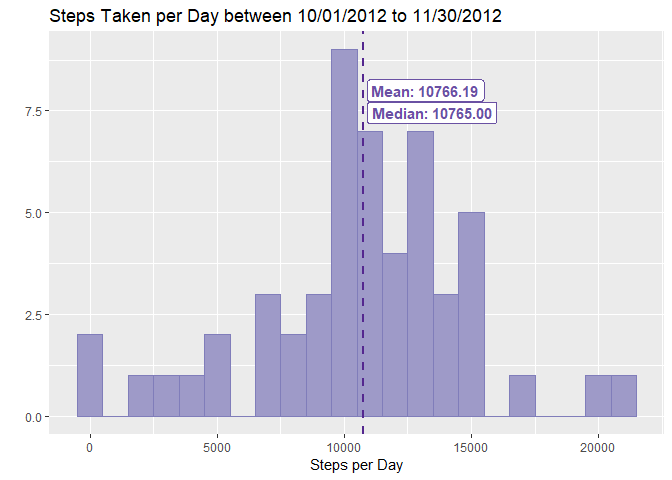
\includegraphics{testing_files/figure-latex/unnamed-chunk-2-1.pdf}

\begin{Shaded}
\begin{Highlighting}[]
\CommentTok{# Step 3:}
\NormalTok{step_mean <-}\StringTok{ }\KeywordTok{round}\NormalTok{(}\KeywordTok{mean}\NormalTok{(per_day}\OperatorTok{$}\NormalTok{steps, }\DataTypeTok{na.rm=}\OtherTok{TRUE}\NormalTok{), }\DecValTok{2}\NormalTok{)}
\NormalTok{step_median <-}\StringTok{ }\KeywordTok{round}\NormalTok{(}\KeywordTok{median}\NormalTok{(per_day}\OperatorTok{$}\NormalTok{steps, }\DataTypeTok{na.rm=}\OtherTok{TRUE}\NormalTok{), }\DecValTok{2}\NormalTok{)}
\KeywordTok{c}\NormalTok{(}\StringTok{"Mean"}\NormalTok{=}\StringTok{ }\NormalTok{step_mean, }\StringTok{"Median"}\NormalTok{ =}\StringTok{ }\NormalTok{step_median)}
\end{Highlighting}
\end{Shaded}

\begin{verbatim}
##     Mean   Median 
## 10766.19 10765.00
\end{verbatim}

\subsubsection{What is the average daily activity
pattern?}\label{what-is-the-average-daily-activity-pattern}

In this section I will:

\begin{enumerate}
\def\labelenumi{\arabic{enumi}.}
\tightlist
\item
  Make a time series plot of the 5-minute interval (x-axis) and the
  average number of steps taken, averaged across all days (y-axis)

  \begin{itemize}
  \tightlist
  \item
    First I will set interval to a factor variable
  \item
    Use aggregate() function to find the mean of steps by the interval
  \item
    Last, I will create the line graph
  \end{itemize}
\item
  Calculate and report which 5-minute interval, on average across all
  the days in the dataset, contains the maximum number of steps
\end{enumerate}

\begin{Shaded}
\begin{Highlighting}[]
\CommentTok{# Step 1:}
\NormalTok{activity}\OperatorTok{$}\NormalTok{interval <-}\StringTok{ }\KeywordTok{as.factor}\NormalTok{(activity}\OperatorTok{$}\NormalTok{interval)}

\NormalTok{per_interval <-}\StringTok{ }\KeywordTok{aggregate}\NormalTok{(activity[}\StringTok{"steps"}\NormalTok{], }\DataTypeTok{by=}\NormalTok{activity[}\StringTok{"interval"}\NormalTok{], mean, }\DataTypeTok{na.rm=}\OtherTok{TRUE}\NormalTok{)}

\KeywordTok{ggplot}\NormalTok{(}\DataTypeTok{data=}\NormalTok{per_interval, }\KeywordTok{aes}\NormalTok{(}\DataTypeTok{x=}\NormalTok{interval, }\DataTypeTok{y=}\NormalTok{steps, }\DataTypeTok{group=}\DecValTok{1}\NormalTok{),}\DataTypeTok{antialias=}\StringTok{"none"}\NormalTok{) }\OperatorTok{+}
\StringTok{      }\KeywordTok{geom_line}\NormalTok{(}\DataTypeTok{color=}\NormalTok{shades[}\DecValTok{2}\NormalTok{],}\DataTypeTok{size=}\NormalTok{.}\DecValTok{8}\NormalTok{) }\OperatorTok{+}
\StringTok{      }\KeywordTok{scale_x_discrete}\NormalTok{(}\DataTypeTok{breaks=}\KeywordTok{seq}\NormalTok{(}\DecValTok{0}\NormalTok{,}\DecValTok{2500}\NormalTok{,}\DataTypeTok{by=}\DecValTok{200}\NormalTok{), }\DataTypeTok{labels=}\KeywordTok{seq}\NormalTok{(}\DecValTok{0}\NormalTok{,}\DecValTok{2500}\NormalTok{,}\DataTypeTok{by=}\DecValTok{200}\NormalTok{)) }\OperatorTok{+}
\StringTok{      }\KeywordTok{xlab}\NormalTok{(}\StringTok{"5-Minute Intervals}\CharTok{\textbackslash{}n}\StringTok{0 to 2455"}\NormalTok{) }\OperatorTok{+}
\StringTok{      }\KeywordTok{ylab}\NormalTok{(}\StringTok{"Average Steps per Day"}\NormalTok{) }\OperatorTok{+}
\StringTok{      }\KeywordTok{ggtitle}\NormalTok{(}\StringTok{"Steps Taken Per 5-Minute Interval"}\NormalTok{,}\DataTypeTok{subtitle=}\StringTok{"Averaged across all days"}\NormalTok{) }\OperatorTok{+}\StringTok{ }
\StringTok{      }\KeywordTok{geom_point}\NormalTok{(}\DataTypeTok{data=}\NormalTok{per_interval,}\KeywordTok{aes}\NormalTok{(}\DataTypeTok{x=}\NormalTok{per_interval}\OperatorTok{$}\NormalTok{interval[}\KeywordTok{which.max}\NormalTok{(per_interval}\OperatorTok{$}\NormalTok{steps)],}
                                      \DataTypeTok{y=}\KeywordTok{max}\NormalTok{(per_interval}\OperatorTok{$}\NormalTok{steps)), }\DataTypeTok{size =} \DecValTok{3}\NormalTok{, }\DataTypeTok{color=}\NormalTok{shades[}\DecValTok{3}\NormalTok{]) }\OperatorTok{+}
\StringTok{      }\KeywordTok{geom_label}\NormalTok{(}\DataTypeTok{data=}\KeywordTok{subset}\NormalTok{(per_interval, interval }\OperatorTok{==}\StringTok{ }\DecValTok{835}\NormalTok{),}
            \KeywordTok{aes}\NormalTok{(interval,steps,}\DataTypeTok{label=}\StringTok{'(853,206)'}\NormalTok{),}\DataTypeTok{nudge_x=}\DecValTok{20}\NormalTok{, }\DataTypeTok{color =}\NormalTok{ shades[}\DecValTok{3}\NormalTok{])}
\end{Highlighting}
\end{Shaded}

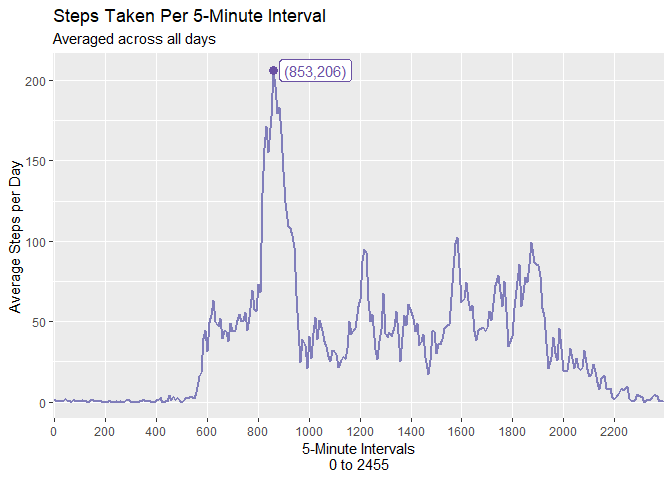
\includegraphics{testing_files/figure-latex/unnamed-chunk-3-1.pdf}

\begin{Shaded}
\begin{Highlighting}[]
\CommentTok{# Step 2:}
\NormalTok{maxInterval <-per_interval[}\KeywordTok{which.max}\NormalTok{(per_interval}\OperatorTok{$}\NormalTok{steps),}\DecValTok{1}\NormalTok{]}
\KeywordTok{setNames}\NormalTok{(}\KeywordTok{as.numeric}\NormalTok{(}\KeywordTok{as.character}\NormalTok{(maxInterval)),}\KeywordTok{c}\NormalTok{(}\StringTok{"Interval with Max Average Steps"}\NormalTok{))}
\end{Highlighting}
\end{Shaded}

\begin{verbatim}
## Interval with Max Average Steps 
##                             835
\end{verbatim}

\subsubsection{Imputing missing values}\label{imputing-missing-values}

In this section I will:

\begin{enumerate}
\def\labelenumi{\arabic{enumi}.}
\tightlist
\item
  Calculate and report the total number of missing values in the dataset
\item
  Devise a strategy for filling in all of the missing values in the
  dataset.

  \begin{itemize}
  \tightlist
  \item
    The stragegy I used is: \textbf{mean per 5-minute interval}
  \end{itemize}
\item
  Create a new dataset that is equal to the original dataset but with
  the missing data filled in.
\item
  Make a histogram of the total number of steps taken each day and
  Calculate and report the mean and median total number of steps taken
  per day.

  \begin{itemize}
  \tightlist
  \item
    Do these values differ from the estimates from the first part of the
    assignment?
  \item
    What is the impact of imputing missing data on the estimates of the
    total daily number of steps?
  \end{itemize}
\end{enumerate}

\begin{Shaded}
\begin{Highlighting}[]
\CommentTok{# Step 1:}
\NormalTok{num_nas <-}\StringTok{ }\KeywordTok{sum}\NormalTok{(}\KeywordTok{is.na}\NormalTok{(activity}\OperatorTok{$}\NormalTok{steps))}
\KeywordTok{c}\NormalTok{(}\StringTok{"Number of NA Values"}\NormalTok{ =}\StringTok{ }\NormalTok{num_nas)}
\end{Highlighting}
\end{Shaded}

\begin{verbatim}
## Number of NA Values 
##                2304
\end{verbatim}

\begin{Shaded}
\begin{Highlighting}[]
\CommentTok{# Step 2:}
\NormalTok{activity_imp <-}\StringTok{ }\NormalTok{activity }\OperatorTok\StringTok{ }\KeywordTok{group_by}\NormalTok{(interval) }\OperatorTok\StringTok{ }
\StringTok{      }\KeywordTok{mutate}\NormalTok{(}\DataTypeTok{steps =} \KeywordTok{ifelse}\NormalTok{(}\KeywordTok{is.na}\NormalTok{(steps), }\KeywordTok{mean}\NormalTok{(steps, }\DataTypeTok{na.rm =} \OtherTok{TRUE}\NormalTok{), steps))}

\CommentTok{# Step 3:}
\NormalTok{activity_imp <-}\StringTok{ }\KeywordTok{as.data.frame}\NormalTok{(activity_imp)}
\NormalTok{num_nas <-}\StringTok{ }\KeywordTok{sum}\NormalTok{(}\KeywordTok{is.na}\NormalTok{(activity_imp}\OperatorTok{$}\NormalTok{steps))}
\KeywordTok{c}\NormalTok{(}\StringTok{"Number of NA Values"}\NormalTok{ =}\StringTok{ }\NormalTok{num_nas)}
\end{Highlighting}
\end{Shaded}

\begin{verbatim}
## Number of NA Values 
##                   0
\end{verbatim}

\begin{Shaded}
\begin{Highlighting}[]
\CommentTok{# Step 4:}
\NormalTok{per_day_imp <-}\StringTok{ }\KeywordTok{aggregate}\NormalTok{(activity_imp[}\StringTok{"steps"}\NormalTok{], }\DataTypeTok{by=}\NormalTok{activity_imp[}\StringTok{"date"}\NormalTok{], sum)}

\KeywordTok{ggplot}\NormalTok{() }\OperatorTok{+}\StringTok{ }\KeywordTok{aes}\NormalTok{(per_day_imp}\OperatorTok{$}\NormalTok{steps) }\OperatorTok{+}\StringTok{ }\KeywordTok{geom_histogram}\NormalTok{(}\DataTypeTok{binwidth=}\DecValTok{900}\NormalTok{, }\DataTypeTok{colour=}\NormalTok{shades[}\DecValTok{2}\NormalTok{], }\DataTypeTok{fill=}\NormalTok{shades[}\DecValTok{1}\NormalTok{]) }\OperatorTok{+}
\StringTok{      }\KeywordTok{geom_vline}\NormalTok{(}\DataTypeTok{xintercept=}\KeywordTok{mean}\NormalTok{(per_day_imp}\OperatorTok{$}\NormalTok{steps), }\DataTypeTok{lwd=}\DecValTok{1}\NormalTok{, }\DataTypeTok{linetype=}\DecValTok{2}\NormalTok{, }\DataTypeTok{color=}\NormalTok{shades[}\DecValTok{4}\NormalTok{]) }\OperatorTok{+}
\StringTok{      }\KeywordTok{geom_label}\NormalTok{(}\DataTypeTok{x=}\DecValTok{13920}\NormalTok{, }\DataTypeTok{y=}\FloatTok{8.65}\NormalTok{, }\KeywordTok{aes}\NormalTok{(}\DataTypeTok{fontface=}\DecValTok{2}\NormalTok{),}\DataTypeTok{color=}\NormalTok{shades[}\DecValTok{3}\NormalTok{], }
                \DataTypeTok{label =} \KeywordTok{paste}\NormalTok{(}\StringTok{'Mean:'}\NormalTok{,}\KeywordTok{format}\NormalTok{(}\KeywordTok{round}\NormalTok{(}\KeywordTok{mean}\NormalTok{(per_day_imp}\OperatorTok{$}\NormalTok{steps), }\DecValTok{2}\NormalTok{), }\DataTypeTok{nsmall =} \DecValTok{2}\NormalTok{))) }\OperatorTok{+}
\StringTok{      }\KeywordTok{geom_label}\NormalTok{(}\DataTypeTok{x=}\DecValTok{14140}\NormalTok{, }\DataTypeTok{y=}\FloatTok{7.7}\NormalTok{, }\KeywordTok{aes}\NormalTok{(}\DataTypeTok{fontface=}\DecValTok{2}\NormalTok{),}\DataTypeTok{color=}\NormalTok{shades[}\DecValTok{3}\NormalTok{], }
                 \DataTypeTok{label =} \KeywordTok{paste}\NormalTok{(}\StringTok{'Median:'}\NormalTok{,}\KeywordTok{format}\NormalTok{(}\KeywordTok{round}\NormalTok{(}\KeywordTok{median}\NormalTok{(per_day_imp}\OperatorTok{$}\NormalTok{steps), }\DecValTok{2}\NormalTok{), }\DataTypeTok{nsmall =} \DecValTok{2}\NormalTok{))) }\OperatorTok{+}
\StringTok{      }\KeywordTok{xlab}\NormalTok{(}\StringTok{"Steps per Day"}\NormalTok{) }\OperatorTok{+}
\StringTok{      }\KeywordTok{ylab}\NormalTok{(}\StringTok{""}\NormalTok{) }\OperatorTok{+}
\StringTok{      }\KeywordTok{ggtitle}\NormalTok{(}\StringTok{"Steps Taken per Day between 10/01/2012 to 11/30/2012"}\NormalTok{)}
\end{Highlighting}
\end{Shaded}

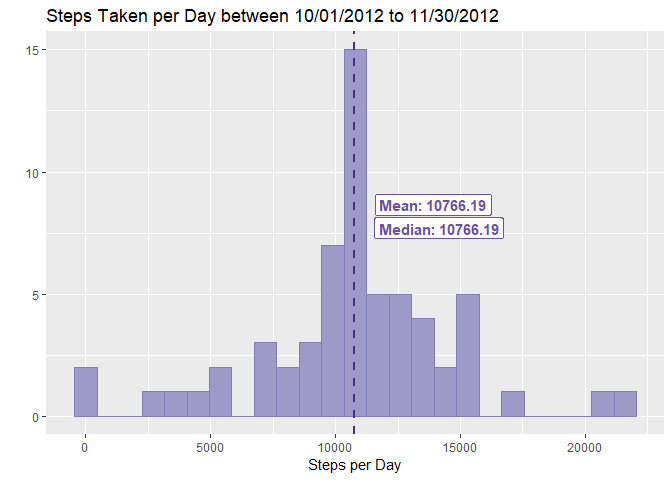
\includegraphics{testing_files/figure-latex/unnamed-chunk-4-1.pdf}

\begin{Shaded}
\begin{Highlighting}[]
\CommentTok{# Step 5:}
\NormalTok{step_mean_imp <-}\StringTok{ }\KeywordTok{round}\NormalTok{(}\KeywordTok{mean}\NormalTok{(per_day_imp}\OperatorTok{$}\NormalTok{steps), }\DecValTok{2}\NormalTok{)}
\NormalTok{step_median_imp <-}\StringTok{ }\KeywordTok{round}\NormalTok{(}\KeywordTok{median}\NormalTok{(per_day_imp}\OperatorTok{$}\NormalTok{steps), }\DecValTok{2}\NormalTok{)}

\NormalTok{r1<-}\StringTok{ }\KeywordTok{c}\NormalTok{(}\StringTok{"Mean"}\NormalTok{=}\StringTok{ }\NormalTok{step_mean, }\StringTok{"Median"}\NormalTok{ =}\StringTok{ }\NormalTok{step_median)}
\NormalTok{r2<-}\StringTok{ }\KeywordTok{c}\NormalTok{(}\StringTok{"Mean"}\NormalTok{ =}\StringTok{ }\NormalTok{step_mean_imp, }\StringTok{"Median"}\NormalTok{ =}\StringTok{ }\NormalTok{step_median_imp)}
\NormalTok{df_imp <-}\StringTok{ }\KeywordTok{rbind}\NormalTok{(r1,r2)}
\KeywordTok{rownames}\NormalTok{(df_imp) <-}\StringTok{ }\KeywordTok{c}\NormalTok{(}\StringTok{'Before Mean Imputation'}\NormalTok{, }\StringTok{'After Mean Imputation'}\NormalTok{)}
\NormalTok{knitr}\OperatorTok{::}\KeywordTok{kable}\NormalTok{(df_imp, }\DataTypeTok{caption =} \StringTok{"Before and After Mean Imputation"}\NormalTok{,}\DataTypeTok{format =} \StringTok{"markdown"}\NormalTok{)}
\end{Highlighting}
\end{Shaded}

\begin{longtable}[]{@{}lrr@{}}
\toprule
& Mean & Median\tabularnewline
\midrule
\endhead
Before Mean Imputation & 10766.19 & 10765.00\tabularnewline
After Mean Imputation & 10766.19 & 10766.19\tabularnewline
\bottomrule
\end{longtable}

\subsubsection{Are there differences in activity patterns between
weekdays and
weekends?}\label{are-there-differences-in-activity-patterns-between-weekdays-and-weekends}

In this section I will:

\begin{enumerate}
\def\labelenumi{\arabic{enumi}.}
\tightlist
\item
  Create a new factor variable in the dataset with two levels -
  ``weekday'' and ``weekend''

  \begin{itemize}
  \tightlist
  \item
    I accomplished this by writing a function called isWeekend that
    returns a factor value of ``weekend'' or ``weekday''
  \end{itemize}
\item
  Make a panel plot containing a time series plot of the 5-minute
  interval (x-axis) and the average number of steps taken, averaged
  across all weekday days or weekend days (y-axis)
\end{enumerate}

\begin{Shaded}
\begin{Highlighting}[]
\CommentTok{# Step 1:}
\NormalTok{isWeekend <-}\StringTok{ }\ControlFlowTok{function}\NormalTok{(dateVar)\{}
\NormalTok{      weekendList <-}\StringTok{ }\KeywordTok{c}\NormalTok{(}\StringTok{"Saturday"}\NormalTok{,}\StringTok{"Sunday"}\NormalTok{)}
      \ControlFlowTok{if}\NormalTok{(}\KeywordTok{weekdays}\NormalTok{(dateVar) }\OperatorTok\StringTok{ }\NormalTok{weekendList) \{}
            \KeywordTok{as.factor}\NormalTok{(}\StringTok{"weekend"}\NormalTok{)}
\NormalTok{      \} }\ControlFlowTok{else}\NormalTok{ \{ }\KeywordTok{as.factor}\NormalTok{(}\StringTok{"weekday"}\NormalTok{) \}}
\NormalTok{\}}

\NormalTok{activity_imp}\OperatorTok{$}\NormalTok{dayType <-}\StringTok{ }\NormalTok{activity_imp}\OperatorTok{$}\NormalTok{date }\OperatorTok\StringTok{ }\KeywordTok{sapply}\NormalTok{(isWeekend) }
\NormalTok{knitr}\OperatorTok{::}\KeywordTok{kable}\NormalTok{(}\KeywordTok{head}\NormalTok{(activity_imp),}\DataTypeTok{caption =} \StringTok{'New variable "dayType" added to dataset'}\NormalTok{,}\DataTypeTok{format =} \StringTok{"markdown"}\NormalTok{)}
\end{Highlighting}
\end{Shaded}

\begin{longtable}[]{@{}rlll@{}}
\toprule
steps & date & interval & dayType\tabularnewline
\midrule
\endhead
1.716981132 & 2012-10-01 & 0 & weekday\tabularnewline
0.339622642 & 2012-10-01 & 5 & weekday\tabularnewline
0.132075472 & 2012-10-01 & 10 & weekday\tabularnewline
0.150943396 & 2012-10-01 & 15 & weekday\tabularnewline
0.075471698 & 2012-10-01 & 20 & weekday\tabularnewline
2.094339623 & 2012-10-01 & 25 & weekday\tabularnewline
\bottomrule
\end{longtable}

\begin{Shaded}
\begin{Highlighting}[]
\CommentTok{# Step 2:}
\NormalTok{per_int_daytyp <-}\StringTok{ }\NormalTok{activity_imp }\OperatorTok\StringTok{ }\KeywordTok{group_by}\NormalTok{(interval,dayType) }\OperatorTok\StringTok{ }\KeywordTok{summarize}\NormalTok{(}\DataTypeTok{mean_steps =} \KeywordTok{mean}\NormalTok{(steps))}
\KeywordTok{names}\NormalTok{(shades) <-}\StringTok{ }\KeywordTok{levels}\NormalTok{(per_int_daytyp}\OperatorTok{$}\NormalTok{dayType)}
\NormalTok{colScale <-}\StringTok{ }\KeywordTok{scale_colour_manual}\NormalTok{(}\DataTypeTok{name =} \StringTok{"dayType"}\NormalTok{,}\DataTypeTok{values =}\NormalTok{ shades)}
\KeywordTok{ggplot}\NormalTok{(per_int_daytyp, }\KeywordTok{aes}\NormalTok{(}\DataTypeTok{x=}\NormalTok{interval, }\DataTypeTok{y=}\NormalTok{mean_steps, }\DataTypeTok{group=}\NormalTok{dayType, }\DataTypeTok{color=}\NormalTok{dayType),}\DataTypeTok{antialias=}\StringTok{"none"}\NormalTok{) }\OperatorTok{+}\StringTok{ }
\StringTok{      }\KeywordTok{geom_line}\NormalTok{(}\DataTypeTok{size=}\NormalTok{.}\DecValTok{8}\NormalTok{) }\OperatorTok{+}\StringTok{ }
\StringTok{      }\KeywordTok{scale_x_discrete}\NormalTok{(}\DataTypeTok{breaks=}\KeywordTok{seq}\NormalTok{(}\DecValTok{0}\NormalTok{,}\DecValTok{2500}\NormalTok{,}\DataTypeTok{by=}\DecValTok{200}\NormalTok{), }\DataTypeTok{labels=}\KeywordTok{seq}\NormalTok{(}\DecValTok{0}\NormalTok{,}\DecValTok{2500}\NormalTok{,}\DataTypeTok{by=}\DecValTok{200}\NormalTok{)) }\OperatorTok{+}
\StringTok{      }\KeywordTok{xlab}\NormalTok{(}\StringTok{"5-Minute Intervals}\CharTok{\textbackslash{}n}\StringTok{0 to 2455"}\NormalTok{) }\OperatorTok{+}
\StringTok{      }\KeywordTok{ylab}\NormalTok{(}\StringTok{"Average Steps per Day"}\NormalTok{) }\OperatorTok{+}
\StringTok{      }\KeywordTok{ggtitle}\NormalTok{(}\StringTok{"Steps Taken Per 5-Minute Interval"}\NormalTok{,}\DataTypeTok{subtitle=}\StringTok{"Averaged across all days"}\NormalTok{) }\OperatorTok{+}
\StringTok{      }\KeywordTok{facet_grid}\NormalTok{(dayType }\OperatorTok{~}\StringTok{ }\NormalTok{.) }\OperatorTok{+}\StringTok{ }\NormalTok{colScale}
\end{Highlighting}
\end{Shaded}

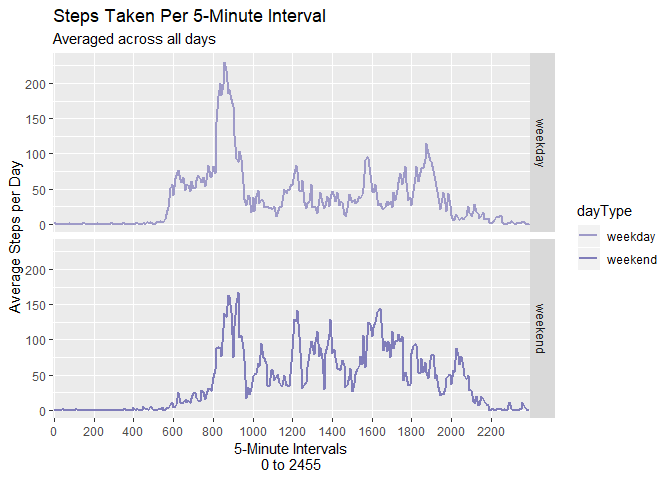
\includegraphics{testing_files/figure-latex/unnamed-chunk-5-1.pdf}


\end{document}
